% ---- pg-506 （书页 494） ----

\begin{mvfigure}
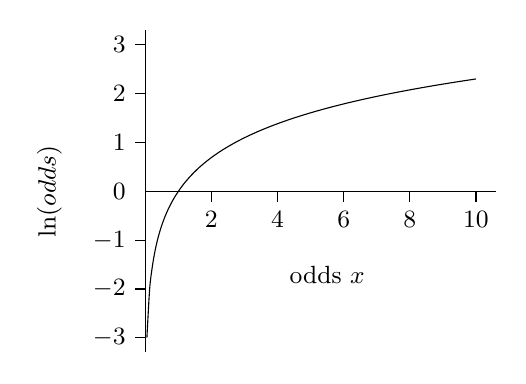
\begin{tikzpicture}[x=0.42cm,y=0.62cm,font=\small]
\draw (0,-3.3)--(0,3.3);
\draw (0,0)--(10.6,0);
\foreach \y in {-3,-2,-1,1,2,3}{\draw (0,\y)--(-0.3,\y) node[left]{$\y$};}
\node[left] at (-0.3,0) {$0$};
\foreach \x in {2,4,6,8,10}{\draw (\x,0)--(\x,-0.22) node[below]{$\x$};}
\draw[domain=0.05:10,samples=120,smooth] plot (\x,{ln(\x)});
\node[rotate=90] at (-2.9,0) {$\ln(\text{odds})$};
\node at (5.5,-1.7) {odds $x$};
\end{tikzpicture}
\phantomsection\label{fig:11.15}\mvcap{图 11.15\quad 机会比的自然对数}
\end{mvfigure}

\phantomsection\label{eq:11-69}
\begin{equation}
\mathrm{logit}(p)=\ln(\mathrm{odds})=\ln\left(\frac{p}{1-p}\right)
\tag{11-69}
\end{equation}
在最简单的模型中, 我们假定 $\mathrm{logit}(p)$ 为预测变量 $Z$ 的线性函数, 即
\phantomsection\label{eq:11-70}
\begin{equation}
\mathrm{logit}(p)=\ln(\mathrm{odds})=\ln\left(\frac{p}{1-p}\right)=\beta_0+\beta_1 z
\tag{11-70}
\end{equation}
由于多数人习惯于用概率思考, 逻辑斯蒂模型可简单表示为
\[
\ln\left(\frac{p}{1-p}\right)=\beta_0+\beta_1 z
\]
先取两边的指数函数, 得到
\[
\theta(z)=\frac{p(z)}{1-p(z)}=\exp(\beta_0+\beta_1 z)
\]
其中 $\exp=\mathrm{e}=2.718$ 为自然对数的底. 再解出 $p(z)$, 得到
\phantomsection\label{eq:11-71}
\begin{equation}
p(z)=\frac{\exp(\beta_0+\beta_1 z)}{1+\exp(\beta_0+\beta_1 z)}
\tag{11-71}
\end{equation}
此函数描述逻辑斯蒂曲线. 概率 $p$ 与预测变量 $z$ 之间的关系不是线性的, 而是如\hyperref[fig:11.16]{图 11.16} 所示, 是一种 S 形曲线. 在\hyperref[fig:11.16]{图 11.16} 中, $\beta_0=-1,\beta_1=2$. 当 $z=0$ 时, 逻辑斯蒂函数的值为 $\exp(\beta_0)/[1+\exp(\beta_0)]$.

\begin{mvfigure}
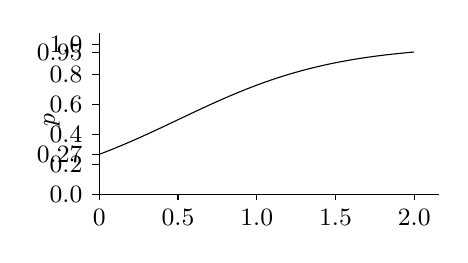
\begin{tikzpicture}[x=2.0cm,y=1.9cm,font=\small]
\draw (0,0)--(0,1.08);
\draw (0,0)--(2.16,0);
\foreach \y/\lab in {0/0.0,0.2/0.2,0.27/0.27,0.4/0.4,0.6/0.6,0.8/0.8,0.95/0.95,1.0/1.0}{\draw (0,\y)--(-0.045,\y) node[left]{$\lab$};}
\foreach \xt in {0,0.5,1.0,1.5,2.0}{\draw (\xt,0)--(\xt,-0.035) node[below]{$\xt$};}
\draw[domain=0:2,samples=120,smooth] plot (\x,{exp(-1+2*\x)/(1+exp(-1+2*\x))});
\node[rotate=90] at (-0.30,0.5) {$p$};
\end{tikzpicture}
\phantomsection\label{fig:11.16}\mvcap{图 11.16\quad 逻辑斯蒂函数($\beta_0=-1,\beta_1=2$)}
\end{mvfigure}
